%!TeX spellcheck = en-US,en-DE
% \documentclass[journal,11pt,draftclsnofoot,]{IEEEtran}
\documentclass[journal,12pt,onecolumn,draftclsnofoot,]{IEEEtran}

%\usepackage[retainorgcmds]{IEEEtrantools}
%\usepackage{bibentry}
\usepackage{xcolor,soul,framed} %,caption

\colorlet{shadecolor}{yellow}
\usepackage[pdftex]{graphicx}
\graphicspath{{../pdf/}{../jpeg/}}
\DeclareGraphicsExtensions{.pdf,.jpeg,.png}

\usepackage[cmex10]{amsmath}
\usepackage{array}
\usepackage{mdwmath}
\usepackage{mdwtab}
\usepackage{eqparbox}
\usepackage{url}
\usepackage{float}

\usepackage[style=numeric,backend=biber]{biblatex}

\addbibresource{\jobname.bib}


\newcommand\blfootnote[1]{%
  \begingroup
  \renewcommand\thefootnote{}\footnote{#1}%
  \addtocounter{footnote}{-1}%
  \endgroup
}

\let\i\textit

% ----------------------------------------------

% Definitions of languages: --------------------
\usepackage{listings}
\lstdefinestyle{cStyle}{
  basicstyle=\scriptsize,
  breakatwhitespace=false,
  breaklines=true,
  captionpos=b,
  keepspaces=true,
  numbersep=5pt,
  showspaces=false,
  gobble=4,
  tabsize=4,
  showstringspaces=false,
  showtabs=false,
}
\renewcommand*{\lstlistingname}{Code}

% ----------------------------------------------

% \hyphenation{op-tical net-works semi-conduc-tor}

%\bstctlcite{IEEE:BSTcontrol}

%=== TITLE & AUTHORS ====================================================================
\begin{document}
\bstctlcite{w}
\title{Python Web Framework}
\author{Carlos~Matheus~Barros~da~Silva$^1$
\\
Igor~Bragaia$^1$
\\
Prof. Lourenço Alves Pereira Jr}
\markboth{INSTITUTO TECNOLÓGICO DE AERONÁUTICA, December~2019
}{}
% ====================================================================
\maketitle

\IEEEpeerreviewmaketitle

% ====================================================================
% ====================================================================
% ====================================================================


% === I. INTRODUCTION ========================================================
% =============================================================================
\section{Objective}
\blfootnote{$^1$Computer Engineering Bachelor Student of ITA}

\IEEEPARstart{T}{h}is project aimed to manipulate HTTP requests on the Application Layer using Python. The project has been made for the Second Bimester Trail of CES35. To manipulate the HTTP requests, the original objective was to create a Python Web Framework, It was conducted following the Rahmonov's tutorial\cite{c1}\cite{c2}\cite{c3}. The Python Web Framework was made to support GET, POST, PUT, DELETE requests, and also supported routing.

After the initial development, we found out that the core implementation that interacts directly with the HTTP request is the Web Server Gateway Interface (WSGI), therefore the project core migrated to the WSGI developed.

The initial activity schedule and planning was:

There won't be a production deploy of the webserver, just localhost.

Activity schedules:

\begin{itemize}
    \item Week 4: Activity planning
    \item Week 5: Study the implementation of the Python Web Framework.
    \item Week 6: Development of basic framework, supporting, at least, HTTP GET requests.
    \item Week 7: Development continuation and finish the presentation content.
    \item Exam Week 1: Creation of final presentation material, including simulation server/client on an application example that uses the developed framework.
\end{itemize}

% ==========================================================================
\section{Project development}
What was developed is a Web Framework written in Python running with WSGI also developed by us. The Web Server Gateway Interface (WSGI) is an stadart interface to connect python web frameworks to a server connection socket and interchange data between the socket and the server framework.

The main idea is that the WSGI creates the HTTP server and provides it an HTTP handler. The HTTP server initiates a socket on that port and starts to listen to an HTTP request. Once it gets a request it passes it to the HTTP handler. The HTTP handler implements the package treatment according to the HTTP protocol, it sets up and read the message headers and handle errors. After that, the handler passes all that treated headers and the package to the server framework itself, from that point it is the server web framework responsibility what will be done regarding that message. After the framework execute what it is to execute to that message, the framework calls the WSGI back with the response message and the WSGI delivers that message back to the client.

This interaction between client, WSGI server and web framework application can be seen in Figure \ref{fig_wsgi}, it represents a sequence diagram of that interaction.

\begin{figure}
  \begin{center}
  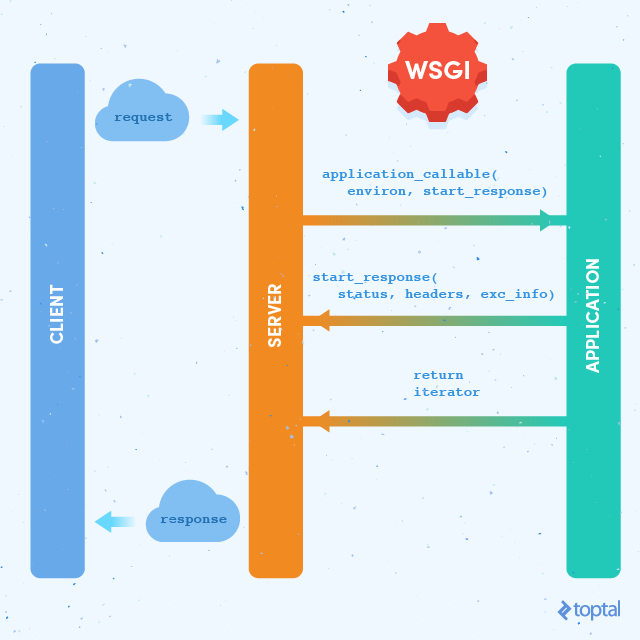
\includegraphics[width=3.0in]{./imgs/wsgi.jpg}
  \caption{WSGI Sequence diagram. The Client sends a message that when it arrives on the host computer it goes to the WSGI HTTP server socket. The WSGI process the message and passes it to the Web Framework application. The web framework processes the message and sends the response message to the WSGI server. The WSGI sends the message back to the client through its HTTP socket.}
  \label{fig_wsgi}
  \end{center}
\end{figure}

The whole interaction between the classes can be seen in Figure \ref{fig_project}, it shows the project classes, interactions, and hierarch.

\begin{figure}
  \begin{center}
  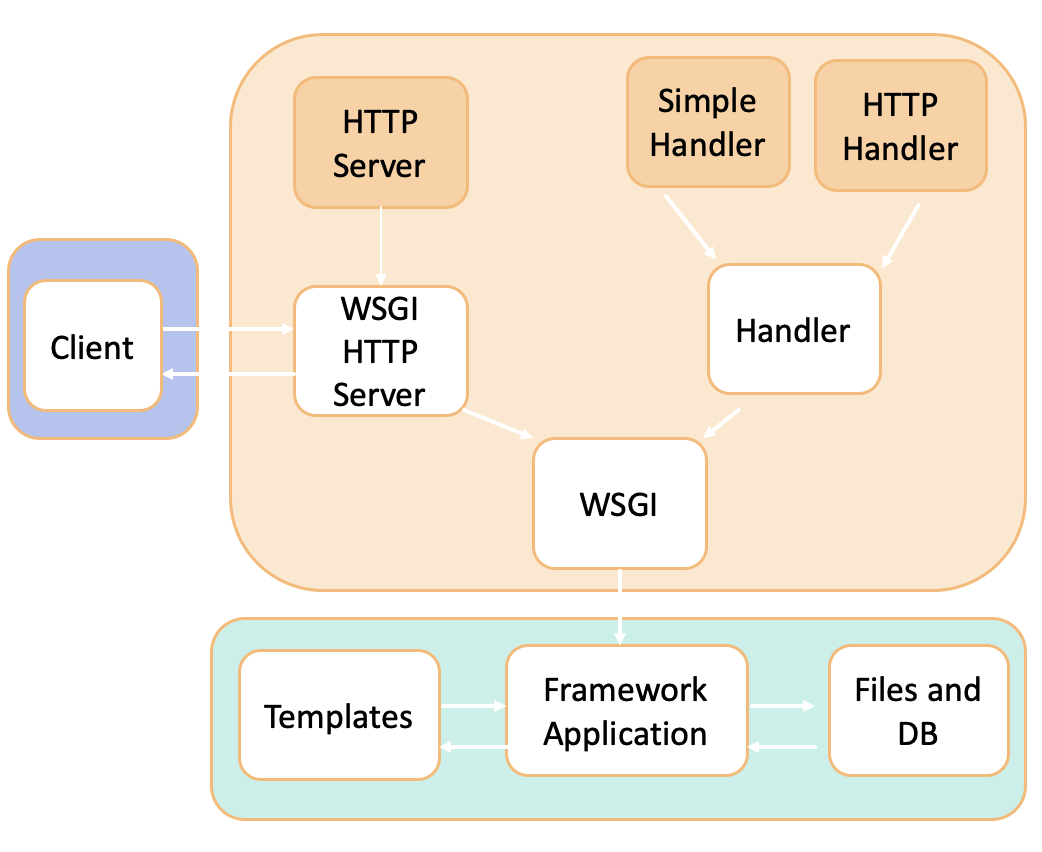
\includegraphics[width=3.0in]{./imgs/project.png}
  \caption{Project Class architecture. The Classes HTTP Server, Simple Handler, HTTP Handler are from standard Python libraries and they perform basic HTTP protocol operations, therefore they were not implemented for the scope of this project and some classes used them or inherited from them.}
  \label{fig_project}
  \end{center}
\end{figure}


%-----------------------------------------------------------------------------
\section{Project validation}
In order to make everything work, both the Python Web framework server and the WSGI were successfully developed and they can be accessed by the \i{Github Repository}$^2$. The usage process can be followed by the repository \i{Readme} file.

\blfootnote{$^2$https://github.com/CarlosMatheus/Python-Web-Framework}

In order to test the code follow the steps:
\begin{itemize}
    \item Clone the repository$^2$.
    \item Make sure to have python3 installed.
    \item Go to the project folder.
    \item Install the project dependencies: ``pip3 install -r requirements.txt''
    \item Run the server python file: ``python3 server.py''
    \item Now you can access the server by ``http://127.0.0.1:8080''
    \item On the example there are the /, /about, and /put\_test\_route routes.
    \item The / route returns a simple text answer with any HTTP method you send to it.
    \item The /about route returns an HTTP web page as an answer to any HTTP method to that route.
    \item The /put\_test\_route route tests the PUT HTTP method and give a different response to the PUT method and it accepts a query. An example would be as shown on Code \ref{code_test_query}.
\end{itemize}

The project also supports HTML files. You just have to put them on the ``templates'' folder as done on the download repository example. As an example, by going to the /about the route it is got an HTML website as shown in Figure \ref{fig_site}.

\begin{figure}
  \begin{center}
  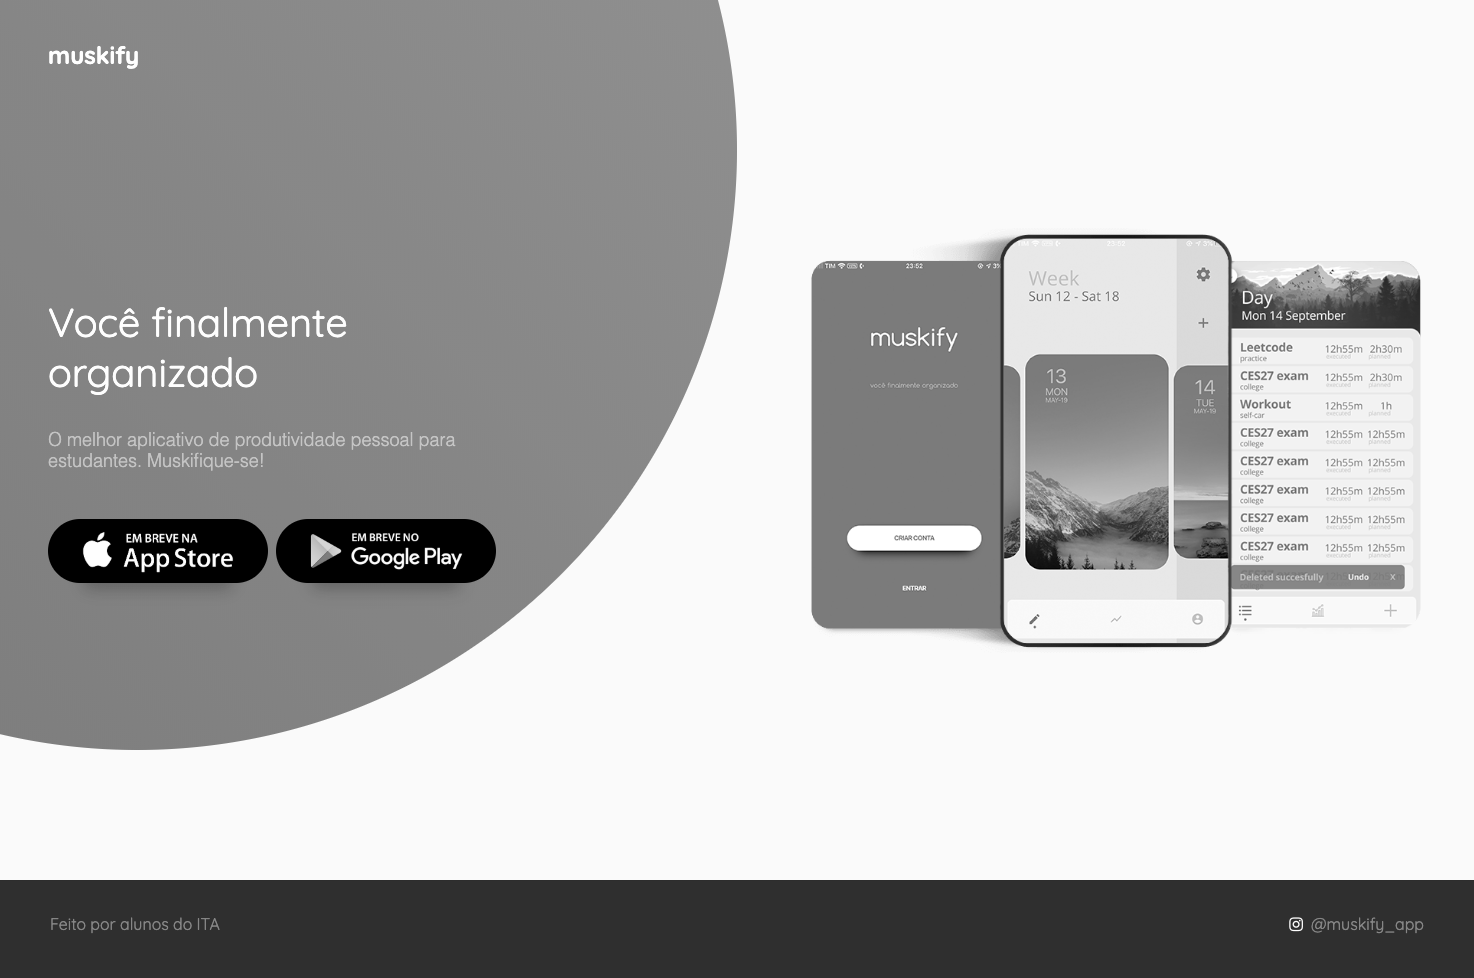
\includegraphics[width=3.0in]{./imgs/example_page.png}
  \caption{Example HTML page with embedded CSS and with images files referencied.}
  \label{fig_site}
  \end{center}
\end{figure}

To summarize all that information it is possible to follow the usage of the Web Framework on the example Code \ref{code_usage}. The usage is simple, just import the Framework and define the routers function using the route decorator as seen on Code \ref{code_decorator}, and then call the start server method.

\lstinputlisting[
    language=python,
    caption={Example of routing decorator.},
    label={code_decorator},
    style=cStyle,
]{./texts/decorator_router.txt}

\lstinputlisting[
    language=python,
    caption={Example server file that uses our Python Web Framework },
    label={code_usage},
    style=cStyle,
]{./texts/usage.py}

\lstinputlisting[
    language=python,
    caption={Test PUT query},
    label={code_test_query},
    style=cStyle,
]{./texts/test_query.txt}


%---------------------------------------------------------------------------
\section{Conclusion}

\subsection{Discussion}
 The project was developed with a good level of deepness both on WSGI implementation and on Web framework implementation. It surely could be improved in a lot of ways, mostly on the web framework side, since it could have better support to CSS files, integration to databases with Models scheme and a lot of other features expected from a web Framework. From the side of the WSGI, it would be possible to implement it deeper and depend less on Python libraries, it would fall on developing many aspects of the HTTP protocol.
 As future improvements, it could be developed better support for HTML templates in general from the Web Framework side, mostly regarding a better integration with different import files like CSS. Today only images are imported correctly.
\subsection{Conclusion}
The work was quite enlightening when it comes to understanding HTTP servers, HTTP handling, WSGI implementation, and the overall workflow of a Web Framework. The results were expresive since the whole project was developed from scratch and in the end, there is a fully functional WSGI connected with a functional Web Framework.

%-------------------------------------------------------------------------

\printbibliography

\vfill
\end{document}

% \begin{figure}
%   \begin{center}
%   \includegraphics[width=2.8in]{./figs/a_star0021.png}
%   \caption{Final state of input from Code \ref{code_input3} after solution.}
%   \label{fig_2}
%   \end{center}
% \end{figure}

% \lstinputlisting[
%     language=python,
%     caption={Small input 3x3.},
%     label={code_input1},
%     style=cStyle,
% ]{./../task2/input1.txt}
